\documentclass[sigconf,screen,nonacm]{acmart}

\setcopyright{none}
\settopmatter{printacmref=false}
\renewcommand\footnotetextcopyrightpermission[1]{}
\acmConference[CS3631 '26]{CS3631 Deep Neural Networks -- Course Project Short Paper}{2026}{University of Moratuwa, Sri Lanka}
\acmYear{2026}
\copyrightyear{2026}

\usepackage{booktabs}
\usepackage{tikz}
\usetikzlibrary{arrows.meta,positioning,fit,backgrounds}

\begin{document}

\title{Trustworthy Deep Learning for Chest X-ray Classification: Progress Toward a Model-Agnostic Shortcut-Suppression Module}

\author{Ravindu Pathirana}
\affiliation{%
  \institution{Department of Computer Science \& Engineering, University of Moratuwa}
  \country{Sri Lanka}}
\email{ravindup.23@cse.mrt.ac.lk}

\author{Kusal Nirukshan}
\affiliation{%
  \institution{Department of Computer Science \& Engineering, University of Moratuwa}
  \country{Sri Lanka}}
\email{kusala.23@cse.mrt.ac.lk}

\author{Dinuka Withanage}
\affiliation{%
  \institution{Department of Computer Science \& Engineering, University of Moratuwa}
  \country{Sri Lanka}}
\email{dinukakeshara.23@cse.mrt.ac.lk}

\author{Sineth Wickramaratna}
\affiliation{%
  \institution{Department of Computer Science \& Engineering, University of Moratuwa}
  \country{Sri Lanka}}
\email{sinethw.23@cse.mrt.ac.lk}

\author{Maleesha Udayanga}
\affiliation{%
  \institution{Department of Computer Science \& Engineering, University of Moratuwa}
  \country{Sri Lanka}}
\email{maleeshau.23@cse.mrt.ac.lk}

\renewcommand{\shortauthors}{Pathirana et al}

\begin{abstract}
Deep learning models have achieved good performance in chest X-ray (CXR) classification, but their predictions may be influenced by text labels, image borders and scanner-related markers instead of the lung regions. Since classification accuracy alone cannot show where the model obtains its evidence, a lightweight Lung-Region Attention module is proposed in this study. The module is placed between a DenseNet121 backbone and its classifier. During training, its attention map is supervised using lung masks, while only the X-ray image is required during inference. Six model variants were evaluated using the same data split and training settings at seed 42, and the baseline and proposed model were further compared across three matched seeds. The proposed model increased Grad-CAM Energy-Inside-Lung by $7.05\pm0.60$ percentage points. No statistically significant accuracy difference was detected between the proposed model and the baseline ($p\geq0.53$). The module adds 131,329 parameters and 0.22\% FLOPs, with measured CPU inference times of $18.44\,\mathrm{ms}$ and $18.45\,\mathrm{ms}$ for the baseline and proposed model, respectively. These preliminary results show an improvement in anatomical localization, but further background-perturbation and external validation experiments are needed before concluding that shortcut reliance has been reduced.

\end{abstract}

\begin{CCSXML}
<ccs2012>
<concept><concept_id>10010147.10010257.10010293.10010294</concept_id><concept_desc>Computing methodologies~Neural networks</concept_desc><concept_significance>500</concept_significance></concept>
<concept><concept_id>10010147.10010257.10010293.10010319</concept_id><concept_desc>Computing methodologies~Image representations</concept_desc><concept_significance>300</concept_significance></concept>
<concept><concept_id>10010405.10010481.10010483</concept_id><concept_desc>Applied computing~Health informatics</concept_desc><concept_significance>300</concept_significance></concept>
</ccs2012>
\end{CCSXML}
\ccsdesc[500]{Computing methodologies~Neural networks}
\ccsdesc[300]{Computing methodologies~Image representations}
\ccsdesc[300]{Applied computing~Health informatics}

\keywords{chest X-ray classification, shortcut learning, lung-region attention, Grad-CAM, attention faithfulness, significance testing, trustworthy deep learning}

\maketitle

\section{Introduction}

Deep learning models have shown good performance on public chest X-ray classification datasets. However, high classification accuracy does not always mean that a model is making its predictions using medically relevant information. A model may achieve a high test accuracy while depending on text markers, image borders or learning different related features that happen to be correlated with a particular class.

This problem has been reported in several previous studies. Zech et al ~\cite{zech2018variable} found that a pneumonia classifier learned information related to the hospital where an image was produced. DeGrave et al ~\cite{degrave2021shortcuts} showed that some COVID-19 chest X-ray models responded to text markers and image borders rather than only to disease-related regions. Oakden-Rayner et al ~\cite{oakdenrayner2020hidden} also showed that a single performance value can hide systematic errors across different patient groups. This behaviour is generally referred to as \emph{shortcut learning} ~\cite{geirhos2020shortcut}. It is difficult to identify from accuracy alone because two models may obtain similar predictions while using very different image regions.

The COVID-19 Radiography Database used in this work combines four classes collected from different sources. Therefore, it is possible that source-specific image properties are correlated with the class labels. Instead of claiming that these shortcuts have already been confirmed in the dataset, we investigate whether the model's Grad-CAM energy \cite{selvaraju2017gradcam} can be moved towards the lung regions. For this purpose, a small residual attention gate is trained using lung-mask supervision. The mask is used only during training, so a segmentation mask is not needed when the trained classifier is used.

The main contributions of this work are:

\begin{itemize}
\item A lightweight residual attention gate supervised using soft lung-mask targets during training, while requiring no mask during inference.

\item A controlled six-arm ablation that separates the effects of mask guidance, attention gating and residual feature preservation. A CBAM spatial-attention branch is also included as a comparison.

\item A paired evaluation of classification performance, Grad-CAM Energy-Inside-Lung and computational cost, with the baseline and proposed model compared across three matched seeds.


\end{itemize}

\section{Related Work}
Most chest X-ray classifiers use established CNN backbones such as ResNet~\cite{he2016resnet} and DenseNet~\cite{huang2017densenet}. CheXNet~\cite{rajpurkar2017chexnet}, for example, demonstrated the effectiveness of DenseNet121 for pneumonia classification. However, strong classification performance does not ensure that these models use clinically relevant image regions when making predictions.

Attention mechanisms have therefore been investigated as a way of improving feature selection and localization. CBAM~\cite{woo2018cbam} learns channel and spatial attention using the classification objective, without explicit anatomical guidance. Tang et al ~\cite{tang2018attention} proposed an attention-guided curriculum for weakly supervised thoracic disease localization. These approaches learn attention mainly from image-level labels and do not directly specify the anatomical region on which the model should focus.

Stronger anatomical guidance has also been considered. Bassi and Attux~\cite{bassi2022segmentation} combined lung segmentation and classification and studied its effect on external generalization. Wei et al ~\cite{wei2022deeppneumonia} used lesion masks to guide hard attention for pneumonia recognition. Mamun et al.~\cite{mamun2026beyond} proposed a CNN--Transformer framework that predicts a soft lung mask and uses it through mask-guided pooling. Debiasing objectives have also been investigated without using anatomical masks. For example, Luo et al~\cite{luo2022pseudobias} inferred pseudo-bias labels for training a bias-balanced chest X-ray classifier.

Therefore, the research gap in this work is not the first use of lung masks for chest X-ray classification. We study a more specific question: whether a lightweight residual gate, supervised using soft lung-mask targets, can shift Grad-CAM energy towards the lungs without requiring a segmentation branch or lung mask during inference. Hard masks and purely multiplicative attention may weaken information near the lung boundary when their estimated attention is incorrect. The proposed residual formulation keeps a direct path for the original features while allowing attended locations to be amplified. The effects of mask guidance and gating are separated through an ablation study. However, performance on severe anatomical distortions, extra-pulmonary abnormalities and external datasets has not been evaluated in this paper.

\section{Proposed Method}

\subsection{Choice of Baseline Backbone}

Four ImageNet-pretrained backbones were compared during the earlier stage of the project, including ResNet50, EfficientNet-B0, ViT-Base/16 and DenseNet121. DenseNet121 achieved the highest classification accuracy in this comparison and was selected as the host backbone for the proposed module. Its training configuration was obtained through a 20-trial Optuna search.

The baseline model, referred to as \textbf{arm A0}, uses the same DenseNet121 backbone and training configuration with the attention module disabled. Therefore, the proposed model and baseline can be compared under consistent training conditions.

\subsection{The Lung-Region Attention Module}
\label{sec:arch}

\begin{figure}[t]
\centering
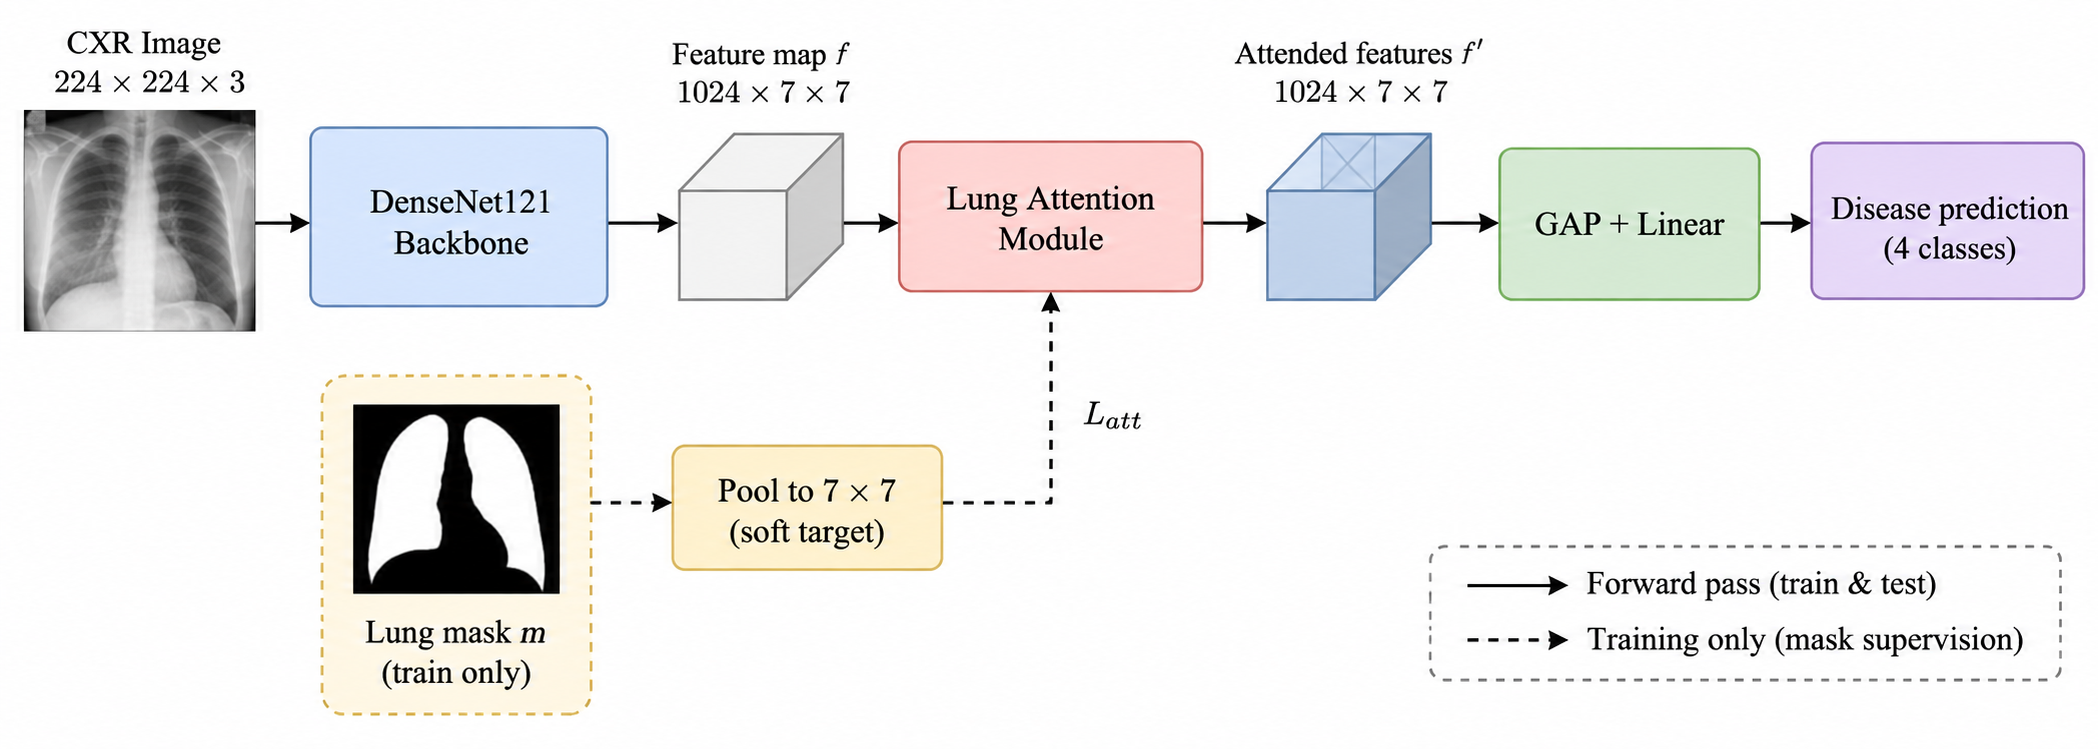
\includegraphics[width=\columnwidth]{figures/Lung Attention module.png}
\caption{The proposed Lung-Region Attention module. A small attention branch produces a spatial map from the backbone features. Lung masks supervise this branch during training, while only the CXR image is required during inference.}
\label{fig:arch}
\Description{A chest X-ray passes through a DenseNet121 backbone to produce a 1024 by 7 by 7 feature map. Two 1 by 1 convolutions, with ReLU and sigmoid activations, produce a single-channel attention map. The map is applied to the features through a residual gate. The resulting features are global-average-pooled and passed to a linear classifier. During training, a lung mask is pooled to 7 by 7 and used to supervise the attention logits.}
\end{figure}

Figure~\ref{fig:arch} presents the structure of the module. For an input CXR image of size $224\times224$, DenseNet121 produces a feature map $f\in\mathbb{R}^{1024\times7\times7}$. The proposed module is inserted between this feature map and the global-average-pooling and classification layers.

\paragraph{Attention-map generation.}
Two $1\times1$ convolutional layers are used to convert the backbone features into a single-channel spatial attention map. A ReLU activation is placed between the convolutions, followed by a sigmoid activation:

\begin{equation}
z = W_2 \ast \operatorname{ReLU}(W_1 \ast f+b_1)+b_2,
\qquad
a=\sigma(z),
\end{equation}

where $z$ denotes the attention logits and $a\in(0,1)^{7\times7}$ is the resulting attention map. The first convolution reduces the feature channels, while the second produces one attention value for each spatial location.

The weights and bias of the second convolution are initialised to zero. This produces a uniform attention value of $a=0.5$ at the beginning of training, allowing the spatial attention pattern to be gradually learned from the data and lung-mask supervision.

\paragraph{Residual attention gate.}
The generated attention map is applied to the backbone features using:

\begin{equation}
f' = f \odot (1+a),
\qquad
\mathbf{s}=h_{\mathrm{cls}}(f'),
\end{equation}

where $\odot$ represents element-wise multiplication, $\operatorname{GAP}$ denotes global average pooling and $\hat{y}$ contains the predicted class logits.

The residual formulation retains the original feature response while allowing locations with higher attention to be amplified. As a result, the contribution of lung-related locations can be increased without fully removing the remaining contextual features. A purely multiplicative version, $f'=f\odot a$, is included as a separate arm in the ablation study to examine the effect of the residual connection.

\paragraph{Mask-supervised training.}
During training, the spatial attention map is guided by the lung mask supplied with each CXR image. The total objective combines the classification loss with an attention-guidance loss:

\begin{equation}
\mathcal{L}
=
\mathrm{CE}_{w}(\hat{y},y)
+
\lambda\mathcal{L}_{\mathrm{att}},
\qquad
\mathcal{L}_{\mathrm{att}}
=
\mathrm{BCE}(z,\tilde{m}).
\end{equation}

where $\operatorname{CE}_{w}$ is the class-weighted cross-entropy loss, $y$ is the true class label and $\lambda$ controls the contribution of attention supervision. The class weight for class $c$ is calculated as:

\begin{equation}
w_c = \frac{N}{K\cdot n_c}.
\end{equation}

where $N$ is the total number of training samples, $K$ is the number of classes and $n_c$ is the number of samples belonging to class $c$.

The target $\tilde{m}$ is obtained by reducing the original lung mask to the $7\times7$ feature resolution using adaptive average pooling. Since the input size is $224\times224$, each pooled value represents the fraction of lung pixels within a corresponding $32\times32$ image region. The resulting target contains continuous values between zero and one, providing soft supervision around the lung boundaries.

The lung mask is used only to calculate $\mathcal{L}_{att}$ during training. During inference, the attention map is generated directly from the backbone features. The trained classifier therefore receives only the CXR image and does not require an additional segmentation stage.

\section{Experimental Setup}

\subsection{Dataset and Split}

The COVID-19 Radiography Database~\cite{chowdhury2020covidradiography, rahman2021enhancement}, hosted on Kaggle\footnote{\url{https://www.kaggle.com/datasets/tawsifurrahman/covid19-radiography-database}}, was used for the experiments. It contains 21,165 CXR images from four classes: COVID-19, Normal, Lung Opacity and Viral Pneumonia. A lung mask is provided for every image.

A stratified 70/15/15 split was used, resulting in 14,815 training images, 3,175 validation images and 3,175 test images. The split was created once, saved and reused in every experiment. Since patient identifiers are not available in the dataset, splitting was performed at the image level.

\subsection{Training Settings}

All images and masks were resized to $224\times224$, and the images were normalised using ImageNet statistics. Identical geometric transformations were applied to each image and its corresponding mask.

Training was completed in two phases. During the first phase, the backbone was frozen and the classification head and attention module were trained for 15 epochs. During the second phase, the final three backbone blocks were unfrozen and the model was fine-tuned for up to 40 epochs. Early stopping was applied after five epochs without validation improvement.

The Adam optimiser was used with learning rates of $4.12\times10^{-3}$ and $6.2\times10^{-5}$ for the two phases. Weight decay was set to $1.87\times10^{-5}$, the batch size was 64 and head dropout was 0.4303. A plateau-based learning-rate scheduler was also applied. These settings were kept unchanged across the compared arms.

The guidance weight $\lambda$ was selected using the validation set. Values from ${0,0.1,0.3,0.5,1.0}$ were evaluated using a shorter training schedule. The largest value that maintained validation macro-F1 within 0.5 percentage points of the unguided reference was selected. Based on this rule, $\lambda=1.0$ was used for the full experiments.

\subsection{Ablation Arms}

Six model variants were evaluated. Four arms form a $2\times2$ comparison of attention gating and lung-mask guidance:

\begin{itemize}
\item \textbf{A0 vanilla}: DenseNet121 without an attention module.
\item \textbf{A1 gate-only}: residual attention gate without mask supervision.
\item \textbf{A4 guidance-only}: mask-supervised attention branch that is not applied to the backbone features.
\item \textbf{A2 full}: residual attention gate with lung-mask supervision.
\end{itemize}

Two additional arms were included. \textbf{A3 multiply-gate} uses $f'=f\odot a$ instead of the proposed residual gate, while \textbf{A5 CBAM spatial} uses the spatial-attention branch of CBAM~\cite{woo2018cbam}. The full six-arm ablation was conducted at seed 42. A0 and A2 were further evaluated using matched seeds 42, 123 and 2026.

\subsection{Evaluation Metrics}

Classification performance was evaluated using accuracy, macro-F1 and macro AUC. McNemar's exact test was used to compare the paired image-level classification outcomes of A0 and A2.

Attention-mask Dice measures the spatial overlap between the module's attention map and the lung-mask target. This metric evaluates whether the learned attention map follows the general lung shape.

Grad-CAM Energy-Inside-Lung (EIL) measures the fraction of Grad-CAM energy located within the lung mask:

\begin{equation}
\operatorname{EIL}(C,M)
=
\frac{\sum_{i,j} C_{ij}M_{ij}}
     {\sum_{i,j} C_{ij}+\epsilon},
\end{equation}

where $C$ is the non-negative normalised Grad-CAM map and $M$ is the lung mask. A higher EIL indicates that a larger proportion of the Grad-CAM energy is located within the lung region. EIL was measured at the feature tensors before and after the attention gate. The Wilcoxon signed-rank test was used to compare paired per-image EIL values on a fixed subset of 1,000 test images.


\section{Results and Discussion}

\subsection{Ablation Results}

\begin{table}[t]
\centering
\footnotesize
\setlength{\tabcolsep}{3pt}
\caption{Seed-42 test results. Accuracy, macro-F1 and Dice use the
full test set ($n=3{,}175$), while EIL uses a fixed subset of 1,000
images. Changes are measured against A0 in percentage points.}
\label{tab:results}

\begin{tabular}{@{}lccccrr@{}}
\toprule
Arm & Acc. & F1 & Dice & EIL & $\Delta$F1 & $\Delta$EIL \\
\midrule
A0 vanilla & 94.68 & 95.11 & -- & 0.296 & ref. & ref. \\
A1 gate-only & 94.52 & 94.97 & 0.080 & 0.284 & $-0.15$ & $-1.21$ \\
A4 guidance & 94.61 & 94.99 & 0.840 & 0.317 & $-0.12$ & $+2.10$ \\
\textbf{A2 full} & \textbf{94.65} & \textbf{95.08}
& \textbf{0.839} & \textbf{0.374}
& \textbf{$-0.03$} & \textbf{$+7.73$} \\
A5 CBAM-S & 94.39 & 94.76 & 0.415 & n/a & $-0.35$ & n/a \\
A3 multiply & 94.24 & 94.46 & 0.840 & n/a & $-0.65$ & n/a \\
\bottomrule
\end{tabular}
\end{table}

Table~\ref{tab:results} presents the seed-42 results. Macro AUC ranged from 0.9922 to 0.9932 and was omitted from the table because only a small variation was observed between the arms.

The baseline A0 obtained 94.68\% accuracy, 95.11\% macro-F1 and an EIL of 0.296. A1, which used the residual gate without mask supervision, produced an attention-mask Dice of 0.080 and an EIL of 0.284. This suggests that adding an attention gate alone was not sufficient to produce lung-aligned attention.

A4 received mask supervision without applying its attention map to the classifier features. It obtained an attention-mask Dice of 0.840, showing that the guidance loss was able to produce a lung-shaped attention map. Its EIL was 0.317, which is an improvement of 2.10 percentage points over A0.

The full A2 model obtained an attention-mask Dice of 0.839 and an EIL of 0.374, corresponding to a 7.73 percentage-point improvement over A0. Its accuracy and macro-F1 were 94.65\% and 95.08\%, respectively. Among the arms for which EIL was measured, the combination of mask supervision and residual gating produced the largest observed improvement.

A3 used purely multiplicative gating and obtained 94.24\% accuracy and 94.46\% macro-F1. A5 used the spatial-attention branch of CBAM~\cite{woo2018cbam} and obtained 94.39\% accuracy, 94.76\% macro-F1 and an attention-mask Dice of 0.415. A3 and A5 were evaluated only at seed 42, and EIL was not computed for these two arms. Their results are therefore treated as supporting single-seed comparisons.

\subsection{Three-Seed Baseline Comparison}

A0 and A2 were evaluated using matched seeds 42, 123 and 2026. Their paired EIL improvements were 7.73, 6.67 and 6.73 percentage points. This gives a mean improvement of $7.05\pm0.60$ percentage points, reported as the mean and sample standard deviation across the three seeds.

The corresponding macro-F1 differences were $-0.03$, $+0.27$ and $-0.49$ percentage points, giving a mean difference of $-0.08\pm0.39$ percentage points. McNemar's exact tests produced $p$-values of 1.000, 0.526 and 0.826 for the three seeds. Therefore, no statistically significant classification-accuracy difference was detected between A0 and A2.

For EIL, Wilcoxon signed-rank tests were conducted using paired per-image values from the fixed subset of 1,000 test images. All three seeds produced $p<10^{-140}$. The percentage of images with improved EIL was 91.9\%, 93.3\% and 91.7\% for seeds 42, 123 and 2026, respectively.

These tests show a consistent image-level EIL increase within the evaluated subset. The Wilcoxon tests describe paired image-level differences within each training run, while the $7.05\pm0.60$ result describes the variation across the three matched seeds.

\subsection{Computational and Qualitative Evaluation}

The proposed module increased the parameter count from 6,957,956 to 7,089,285, adding 131,329 parameters or 1.89\%. Computational cost increased from 2.8645 to 2.8710 GFLOPs, corresponding to a 0.22\% increase at an input size of $224\times224$. Under the reported CPU benchmark, inference times were 18.44,ms for A0 and 18.45,ms for A2.

\begin{figure}[t]
\centering
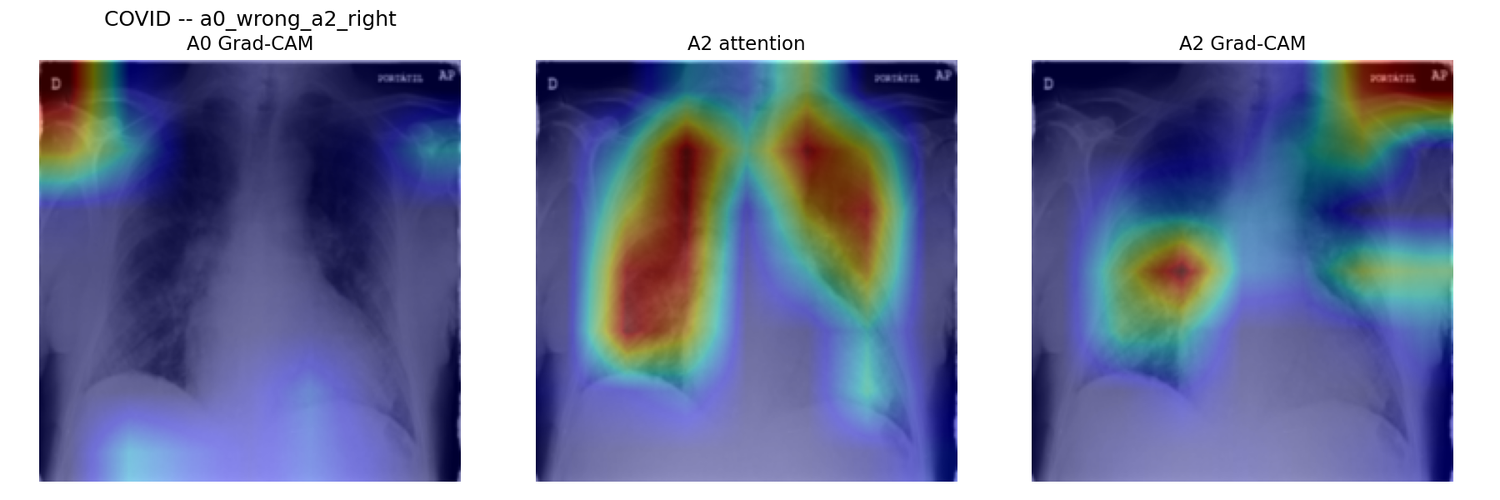
\includegraphics[width=\columnwidth]
{figures/covid_shortcut_example_crop.png}
\caption{A COVID-19 test image misclassified by A0 but correctly classified by A2. The A0 Grad-CAM response is concentrated near the ``PORTABLE AP'' marker, while A2 places more Grad-CAM evidence within the lung region.}
\label{fig:shortcut}
\Description{Three panels showing one COVID-positive test image. The first panel shows the A0 Grad-CAM response near the PORTABLE AP acquisition marker. The second panel shows the attention map produced by A2 within the lung fields. The third panel shows the A2 Grad-CAM response located mainly within the lungs.}
\end{figure}

Figure~\ref{fig:shortcut} presents an example in which A0 places a large part of its Grad-CAM response near the ``PORTABLE AP'' acquisition marker. This is similar to the shortcut behaviour discussed by DeGrave et al.~\cite{degrave2021shortcuts}. For the same image, A2 places more Grad-CAM energy within the lungs and produces the correct classification. This example illustrates the type of localization change measured by EIL, although one example cannot establish the overall behaviour of the model.

\begin{figure}[t]
\centering

\includegraphics[width=0.62\columnwidth]
{figures/attention_grid.png}
\caption{Example attention maps produced by A2 for the four classes. Lung-shaped attention patterns can be observed across the presented images.}
\label{fig:grid}
\Description{A four-by-four grid of chest X-ray images with attention-map overlays. The rows contain examples from the COVID-19, Lung Opacity, Normal and Viral Pneumonia classes. Most high-attention regions appear within the lung fields.}
\end{figure}

Additional attention maps are presented in Figure~\ref{fig:grid}. Lung-shaped attention patterns can be observed for examples from COVID-19, Lung Opacity, Normal and Viral Pneumonia. These qualitative examples support the attention-mask Dice measurements, while the EIL results provide the main quantitative comparison of evidence placement.

\section{Limitations and Ongoing Work}

Several limitations should be considered when interpreting the results. The dataset does not provide patient identifiers, so the data were divided at the image level rather than the patient level. It is therefore possible that images belonging to the same patient appear in different partitions. DenseNet121 was also selected during an earlier backbone comparison that used the current nominal test partition. The reported classification performance should therefore be confirmed using an untouched external dataset.

The attention map has a resolution of $7\times7$, with each cell representing an approximately $32\times32$ region of the input image. The soft mask targets provide some boundary information, but small abnormalities and detailed lung boundaries may not be represented precisely at this resolution.

Only A0 and A2 were evaluated across three matched seeds. The complete six-arm ablation was conducted at seed 42, and EIL was not computed for A3 and A5. Further repeated evaluations would provide a more complete comparison of the attention variants.

The current experiments measure where the model's Grad-CAM energy is located. Although EIL increased, this does not directly prove that the classifier depends less on background information~\cite{adebayo2018sanity}. Lung-preserving background perturbations are currently being investigated to measure this more directly. Future work will also include external validation, additional CNN backbones, adaptation to ViT feature representations and evaluation using independently generated lung masks. Multi-scale or pathology-adaptive attention targets may also be studied to better represent small findings and changes near the lung boundaries.

\section{Conclusion}

A lightweight Lung-Region Attention module was presented for DenseNet121-based chest X-ray classification. The module uses soft lung-mask supervision during training and applies the learned attention through a residual gate, while no mask is required during inference. In the seed-42 ablation, the full model increased Grad-CAM Energy-Inside-Lung by 7.73 percentage points over the baseline. Across three matched seeds, the mean improvement was $7.05\pm0.60$ percentage points. No statistically significant accuracy difference was detected between the proposed model and the baseline, while the module added 1.89\% parameters and 0.22\% FLOPs. These results show that the proposed approach can improve lung-region evidence localization with a small computational increase. Further evaluation is being carried out to determine whether the observed localization improvement also reduces dependence on background shortcuts and generalizes to other datasets and model architectures.


\bibliographystyle{ACM-Reference-Format}
\bibliography{references}

\end{document}
